\subsubsection{Biomeolecular Modeling}
\index{Zacharias, Martin}

\paragraph{Research Team}
%
Martin Zacharias (Professor), Andr\'{e} Barthel (Postdoc), Andreas May (PhD Student), Florian Sieker (PhD Student), J\'{e}r\'{e}my Curuksu (PhD Student), Srinivasaraghavan Kannan (PhD Student)\\


The research focus of the Computational Biology group is the study of biomolecular
association and conformational flexibility using computer simulation approaches.
The simulation studies are aimed to better understand structure formation of
biomolecules and the mechanism of ligand-receptor association. As the major
computational tool we employ the molecular dynamics simulation method to investigate
the structure and dynamics of proteins and nucleic acids at atomic resolution.
We also develop new docking approaches that allow to predict putative binding sites
for ligands and inhibitors on the surface of biological target molecules.
The prediction of putative ligand binding geometries and binding sites on a
biomolecule is of tremendous importance for the design of new drugs that can bind
and interfere with the function of biomolecules. Focus of another research area is
to improve comparative protein structure modeling. Improving the accuracy of
structural modeling of proteins is also of central importance to use such structural
models for drug design. In close collaboration with experimental groups the
computational approaches are applied to several biologically important targets.

\paragraph{Highlights}

\null{\sl Conformational Dynamics of Nucleic Acids }

The conformational flexibility of DNA is central to its many biological functions including recognition by proteins during gene regulation, DNA repair, packaging in the cell and transient melting during transcription and replication. Specific binding by proteins is not only determined by specific interactions between DNA and proteins but also by the sequence-dependent structure and deformability of the DNA helix. The DNA twist flexibility is of particular importance since it plays a role during supercoiling and packing of DNA. We have designed a method to induce twist deformations in DNA during simulations and to record associated free energy changes. Simulations allowed to extract free energy profiles for twist deformations and were performed on a series of DNA dodecamer duplexes. The shape of the free energy curves was similar for all duplexes. The calculated twist deformability was in good agreement with experiment and showed only modest variation for the complete duplexes. However, the response of the various base pair steps on twist stress was highly non-uniform. In particular, pyrimidine/purine steps were much more flexible than purine/purine steps followed by purine/pyrimidine steps. This non-uniform local response may significantly alter the shape of the DNA recognition surface which in turn can affect binding of proteins and other ligands as a result of external twist stress. It was also possible to extract correlations of twist changes and other helical as well as global parameters of the DNA molecules. Severe un-twisting of DNA below an average of 25 degrees per base-pair step resulted in the onset of a global structural transition with a significantly smaller twist at one end of the DNA compared to the other end. (Fig.~\ref{fig:twist}) The effect of DNA damage and binding of ligands on the twist deformability will be subject of future studies.


\begin{figure}[ht]
  \begin{center}
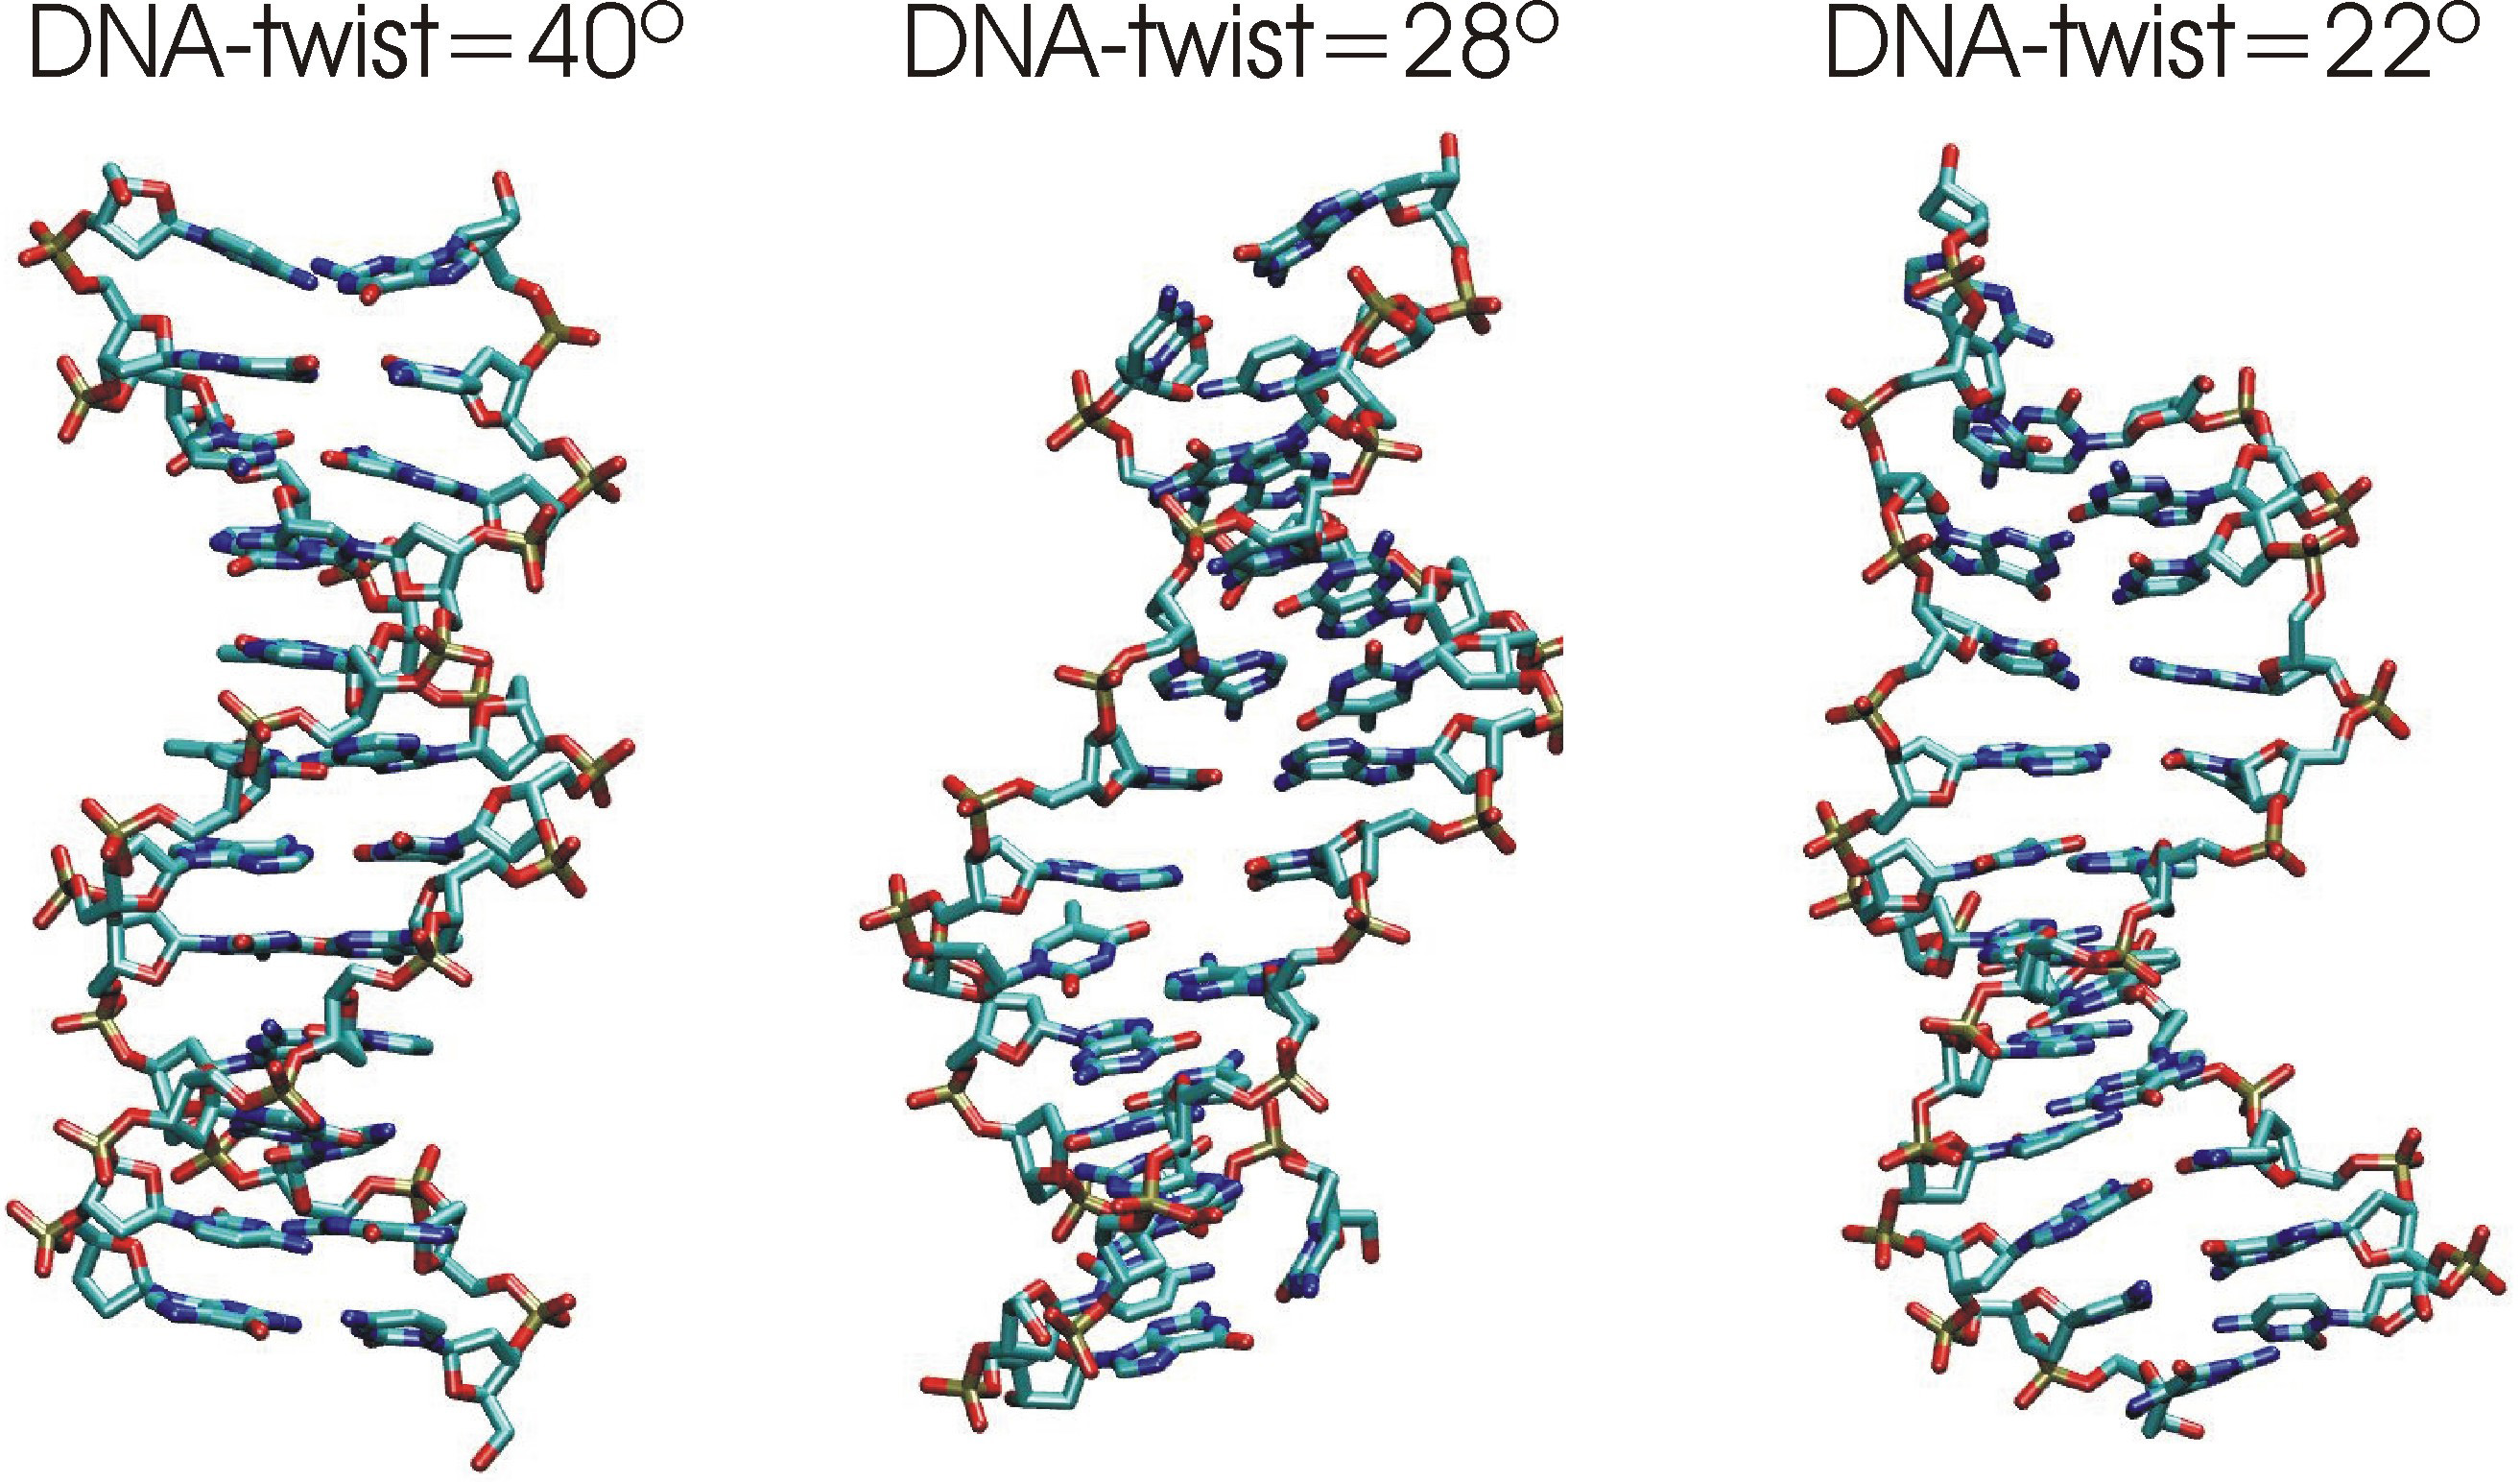
\includegraphics[width=\hsize]{Zacharias/figure_Zacharias_2006.png}
    \mycaption{Overtwisting and untwisting of DNA during molecular dynamics simulations. Explicit solvent molecular dynamics simulations were performed on 12 base pair DNA molecules including a penalty potential for modifying the average DNA twist between 40 degrees (left panel) and 22 degrees (right panel). At twist angles below 25 degrees the DNA splits into a near B-DNA region and a region with average twist of 12 degrees. DNA molecules represent simulation snapshots and are shown as atom color coded stick models. }
       \label{fig:twist}
  \end{center}
\end{figure}

{\sl Flexible Docking of protein-ligand complexes}
\null
Biomolecular association can involve conformational changes of the binding partners. In order to predict the structure of biomolecule complexes using computational docking methods it is necessary to appropriately account for such conformational changes during the simulation. One of our research projects specifically focuses on better accounting for conformational flexibility during docking. A major step that we achieved was the development and testing of a new method to efficiently account for global backbone motions of proteins during protein-protein and protein-ligand docking. In this approach induced fit conformational changes are based on
relaxing the protein conformation in soft collective degrees of freedom of the protein. The flexible global degrees of freedom can be calculated rapidly prior to docking. Very promising results have been achieved on several test systems indicating that this could be a new route for efficient flexible molecular docking. The possibility to use this method to rapidly extract potential drug-like molecules from a data base and identify putative binding sites on protein molecules will be explored in future studies.


\myparagraph{Collaborations}
%
Bremen Area Collaborations:
\begin{enumerate}
\item {\sl International University Bremen}\\Prof. K. Brix \\ Models for Protease Trafficking
\\Prof. F.O. Gl�ckner \\ Sulfatases
\\ Prof. M.-Th. H�tt  \\Topology of protein interaction networks
 \\ Prof. A. Jeltsch  \\ Simulation of enzyme dynamics
\\ Prof. G. Muskhelishvili \\ Molecular modeling
\\Prof. W. Nau\\ Dynamics of end-to-end Contact Formation of Small Peptides
\\Prof. U. Schwaneberg and Dr. D. Roccatano \\Influence of Organic Cosolvents on the Industrially Important Enzyme P450 BM-3
\\Prof. S. Springer\\Conformational Flexibility of MHC Class I Molecules in Ligand-bound and Free States
\end{enumerate}
National \& International Collaborations:
\begin{enumerate}
\item {\sl Technische Universit�t Darmstadt}\\Prof. H.U. G�ringer\\Modeling serum stable RNA aptamers
\item {\sl Institute for Biophysics, Brno, Tschec Rep.}\\Dr. J. Sponer \\Conformational dynamics of RNA
\item {\sl IBPC Paris}\\Dr. C. Prevost\\New Docking Methods
\end{enumerate}
\null
%
\paragraph{Grants}
\begin{enumerate}
\item Funded by DFG, \emph{Protein Protein Docking}, DFG 153/5-1,
(October 2004 - September 2007) \item Funded by DFG, \emph{RNA
Peptid Wechselwirkung}, DFG 153/11-1, (April 2006 - March 2008)
\item Funded by Volkswagenstiftung,  \emph{Replica Exchange},
(January 2005 - December 2007) \item Funded by US Department of
Energy, \emph{US Computational Grande Challenge Project:
Biomolecular Simulation of Base Excision Repair and Protein
Signaling, Pacific Northwest National Laboratory}
\end{enumerate}

\newpage
\paragraph{Other Support Grants}
\begin{enumerate}
\item Cotutelle support grant for PhD student J\'{e}r\'{e}my
Curuksu, Universit\'{e} Franco-Allemande (UFA)
\item Cotutelle support grant for
PhD student Adrian Saladin, Universit\'{e} Franco-Allemande (UFA)
\end{enumerate}

\nocite{Zacharias1,Zacharias2,Zacharias3,Zacharias4,Zacharias5,Zacharias6,Zacharias7,Zacharias8,Zacharias9,Zacharias10,Zacharias11,Zacharias12,Zacharias13,Zacharias14,Zacharias15}
